\chapter{Laboratorio de prácticas}
\label{laboratorio}
\section{Herramientas hardware} % Herramientas Hardware
En este punto se resumen las características de los dispositivos utilizados:
\\\\$\blacksquare$ {\underline{\textbf{Placa Sniffer - Api-Mote (V4 Beta)}}}
\\\\La placa Api-Mote es un dispositivo híbrido diseñado para la interacción de bajo nivel con el estándar IEEE 802.15.4 y el protocolo de radio Zigbee. Con este dispositivo se puede evaluar la seguridad de una red IEEE 802.15.4/Zigbee, capturando información,  inyectando paquetes y retransmitiendo datos a la red.
\begin{figure}[H]
\centering
\subfloat[Vista anterior]{
\includegraphics[width=7cm]{figuras/apimotefront.eps}}
\subfloat[Vista posterior]{
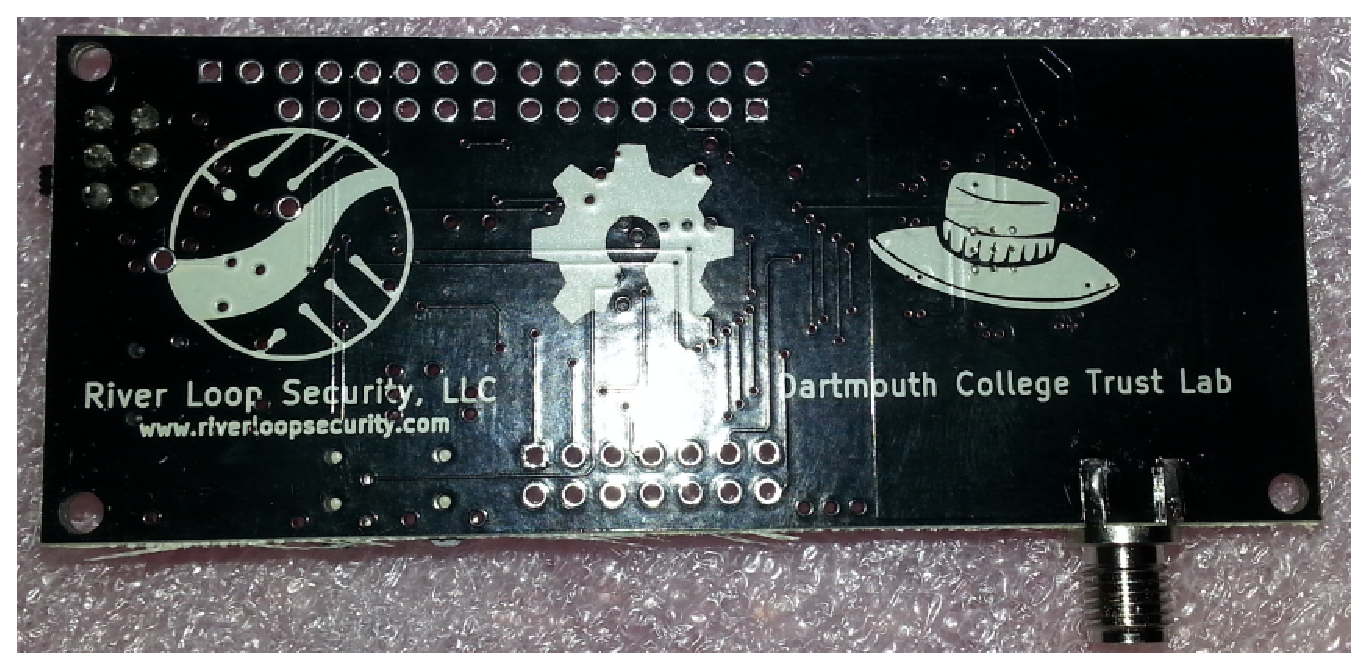
\includegraphics[width=7cm]{figuras/apimoteback.eps}}
\caption{Placa Sniffer Api-Mote (V4-Beta), protocolo IEEE 802.15.4/Zigbee \cite{apimote}}
\label{apimote}
\end{figure}
Las especificaciones técnicas de una placa Api-Mote, son las siguientes:
\begin{itemize}
\item Transceptor de RF compatible con IEEE 802.15.4 de 2.4 GHz y ZigBee Ready (CC2420).
\item Interoperabilidad con otros dispositivos IEEE 802.15.4.
\item MCU de 16 bits de potencia ultrabaja (116kB Flash, 8KB RAM) (MSP430F2618), con ADC integrado, DAC, supervisor suministro de voltaje y controlador DMA.
\clearpage
\item Programación y recolección de datos vía USB.
\item Bajo consumo.
\item Se soporta cifrado y autenticación hardware de enlace de datos.
\item Soporte de firmware básico basado en GoodFET.
\end{itemize}
\vspace{1cm}
$\blacksquare$ {\underline{\textbf{Dispositivos Zigbee}}}
\\\\Actualmente hay muchos fabricantes que han desarrollado dispositivos Zigbee centrados en domótica como Philips, Xiaomi, Ksix y Samsung entre otros. Para este proyecto se ha decidido utilizar los sensores de Ksix ya que el desarrollo de dispositivos IoT Zigbee por parte de este fabricante es reciente y no se han encontrado otros proyectos de auditoría de seguridad en los que se analizaran estos dispositivos:
\begin{itemize}
\item Puerta de enlace Zigbee: permite configurar escenas inteligentes y automatizaciones para determinar el comportamiento de los sensores y los dispositivos conectados a una red.
\item Sensor de movimiento: gracias a este sensor es posible recibir notificaciones de los movimientos detectados en una habitación.
\item Sensor para puertas y ventanas: con este sensor es posible llevar un registro en un smartphone de los momentos en que las puertas y las ventanas se abren o se cierran.
\item Cámara IP con detector de movimiento: permite recibir notificaciones de cualquier movimiento en tiempo real.
\end{itemize}
\begin{figure}[H]
\centerline{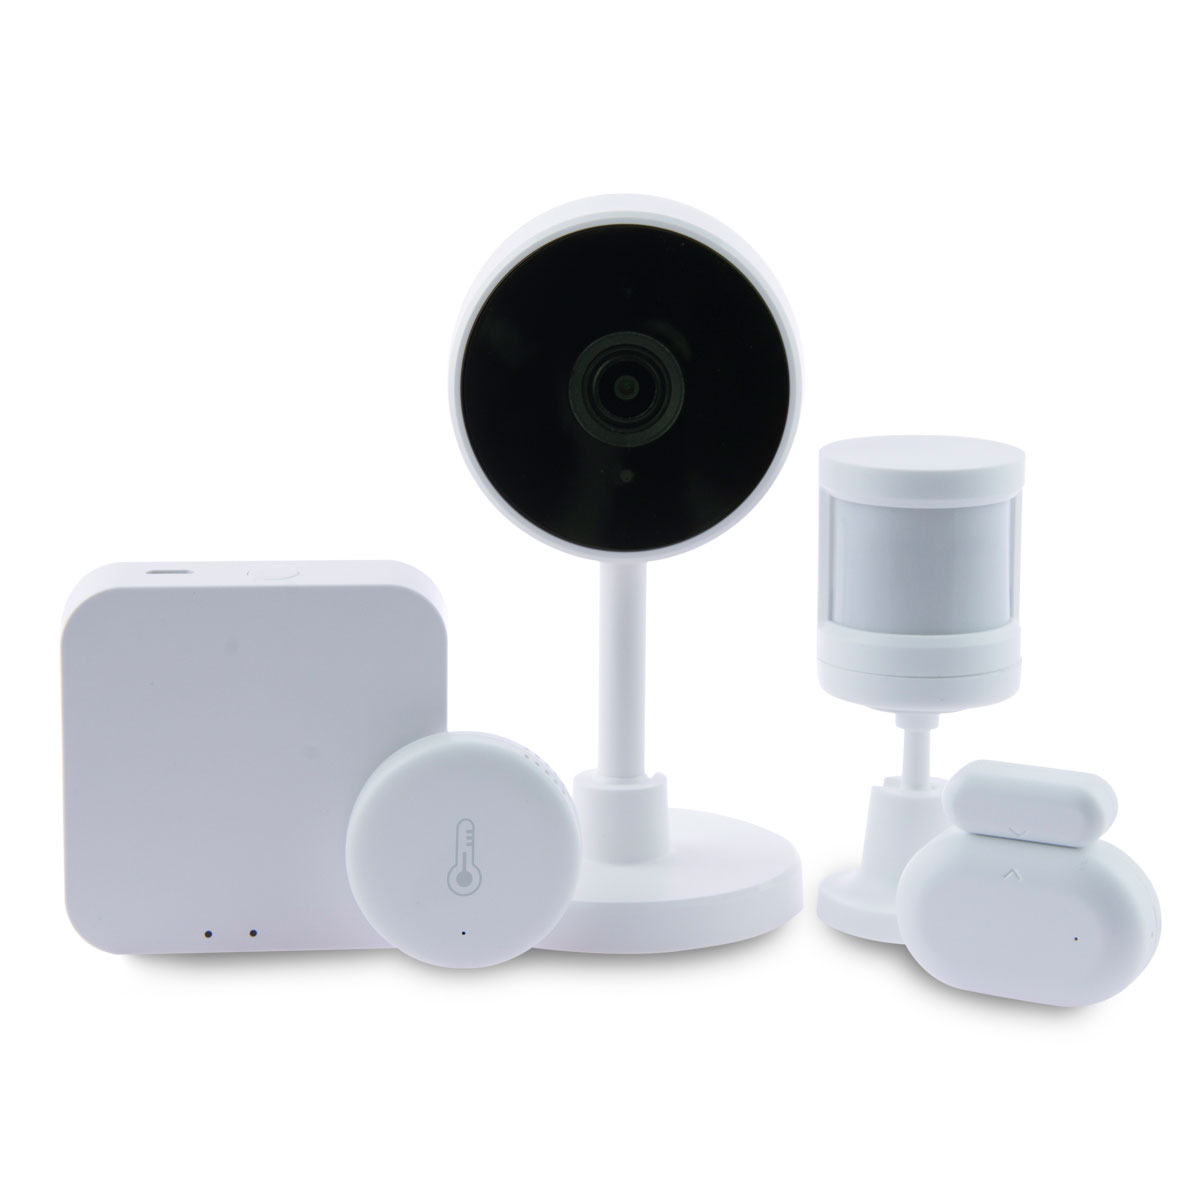
\includegraphics[width=7cm]{figuras/ksisdevices.jpg}}
\caption{Dispositivos IoT Zigbee (fabricante Ksix) \cite{dispositivosksix}}
\end{figure}
\clearpage




\section{Herramientas software} % Herramientas Software
Para llevar a cabo la auditoría de seguridad sobre el protocolo Zigbee, han sido necesarias las siguientes herramientas software:
\\\\$\blacksquare$ {\underline{\textbf{Wireshark}}}
\\\\Wireshark es el analizador de protocolos de red más utilizado a nivel mundial. Su función principal es el análisis de redes de comunicación y la solución de problemas existentes en ellas. Esta herramienta permite ver todo el tráfico que pasa a través de una red usándose para capturar y analizar el tráfico IEEE 802.15.4/Zigbee.
\\\\ Wireshark es una aplicación multiplataforma y en el caso de la distribución Kali Linux (debian) se instala de la siguiente forma:
\\\\\# apt-get install wireshark
\\\\$\blacksquare$ {\underline{\textbf{KillerBee y Attify Zigbee Framework}}}
\\\\KillerBee es un framework desarrollado en python y diseñado para auditar redes IEEE 802.15.4 y Zigbee. Mientras que, Attify Zigbee Framework es una aplicación gráfica para utilizar las herramientas de KillerBee simplificando su uso. Con este framework se puede capturar tráfico en redes Zigbee, retransmitir el tráfico capturado, atacar los sistemas criptográficos, etc. 
\\\\Entre las herramientas que incluye el framework, se destacan las siguientes:
\begin{itemize}
\item zbfind: permite rastrear la localización de los transmisores IEEE 802.15.4.
\item zbstumbler: herramienta de descubrimiento de redes IEEE 802.15.4 y Zigbee activas.
\item zbdump: captura tramas IEEE 802.15.4 y las almacena en un archivo para su posterior análisis.
\item zbdsniff: captura el tráfico ZigBee en busca de tramas de red y envío de claves inalámbricas.
\item zbreplay: implementa un ataque de repetición, retransmitiendo el tráfico de red capturado desde un archivo.
\item zbassocflood: intenta saturar una red enviando peticiones constantes de asociación.
\item zbrealign: falsifica una trama de reasociación PAN desde el coordinador a un dispositivo objetivo.
\end{itemize}
\clearpage
Como se indica en el repositorio de github, es necesario tener instaladas una serie de dependencias de python como pyusb, pycrypto o scapy. La herramienta se instala correctamente de la siguiente forma:
\\\\\# dnf install pygtk2 pycairo pyusb pycrypto pyserial python-devel libgcrypt-devel
\\\# git clone https://github.com/secdev/scapy \&\& cd scapy
\\\# python setup.py install
\\\# git clone https://github.com/riverloopsec/killerbee \&\& cd killerbee
\\\# python setup.py install
\\\\$\blacksquare$ {\underline{\textbf{Nmap}}}
\\\\Nmap es una herramienta de código abierto que sirve para efectuar escaneo de redes. Nmap puede enviar diferentes tipos de paquetes para determinar qué hosts están disponibles en la red, qué servicios (nombre y versión de la aplicación) ofrecen esos hosts, qué sistemas operativos (versiones de SO) están ejecutando, qué tipo de filtros de paquetes / firewalls están en uso y otras características. Nmap es una aplicación multiplataforma y en el caso de la distribución Kali Linux (debian) se instala de la siguiente forma:
\\\\\# apt-get install nmap
\section{Red industrial Zigbee} % Red industrial Zigbee (laboratorio)
Para el estudio de la seguridad del protocolo Zigbee, utilizando las herramientas hardware y software descritas anteriormente, se ha creado un laboratorio de trabajo con la siguiente configuración:
\begin{itemize}
\item Se ha instalado la puerta de enlace Zigbee dentro de una red Wifi, actuando como coordinador de la red.
\item Se han conectado los dos sensores IoT de Ksix (sensor para puertas y sensor de movimiento) y la cámara ip directamente al coordinador Zigbee formando una topología de red en estrella.
\item Se ha instalado la aplicación TuyaSmart en un smartphone para controlar la red Zigbee y las alertas de los sensores.
\item Se ha establecido un modelo de seguridad centralizado en la red, adoptando una política de seguridad en modo residencial.
\item Se ha establecido un modelo de comunicación IoT de dispositivo a puerta de enlace.
\item Se han instalado las herramientas de pentesting especificadas anteriormente en un ordenador con la distribución Kali Linux (distribución orientada a audiorías de seguridad), al cual se le ha conectado la placa sniffer Api-Mote.
\end{itemize}
\clearpage